% !TEX root = platooning.tex
\section{Problem Formulation \label{sec:formulation}}
\subsection{Vehicle Dynamics}
Consider a UAV whose dynamics are given by
\begin{equation}
\dot{x} = f(x,u)
\end{equation}

\noindent where $x\in\mathbb{R}^n$ represents the state, and $u\in\mathbb{R}^{n_u}$ represents the control action. In this paper, we will assume that each vehicle has a simple kinematics model of a quadrotor:

\begin{equation} \label{eq:dyn}
\begin{aligned}
\dot{p}_x &= v_x, \qquad \dot{p}_y = v_y  \\
\dot{v}_x &= u_x, \qquad \dot{v}_y = u_y, \qquad |u_x|,|u_y| \le u_\text{max}
\end{aligned}
\end{equation}

\noindent where the state (at a fixed altitude) $x=(p_x, v_x, p_y, v_y)\in\mathbb{R}^4$ represents the quadrotor's position in the $x$ direction, its velocity in the $x$ direction, and its position and velocity in the $y$ direction, respectively. For convenience, we will denote the position and velocity $p=(p_x, p_y),v=(v_x,v_y)$, respectively. We will consider a group of $N$ quadrotors $Q_i, i=1\ldots,N$.

In general, the problem of collision avoidance among $N$ vehicles cannot be tractably solved using traditional dynamic programming approaches because the computation complexity of these approaches scales exponentially with the number of vehicles. Thus, in our present work, we will consider the situation where $N$ quadrotors form a platoon. The structure imposed by the platoon enables us to analyze the liveness and safety of the quadrotors in a tractable manner.

\subsection{Relative Dynamics and Augmented Relative Dynamics}
Besides \eqref{eq:dyn}, we will also consider the relative dynamics between two quadrotors $Q_i,Q_j$. These dynamics can be obtained by defining the relative variables

\begin{equation} \label{eq:rel_var}
\begin{aligned}
p_{x,r} &= p_{x,i} - p_{x,j}, \qquad p_{y,r} = p_{y,i} - p_{y,j}\\
v_{x,r} &= v_{x,i} - v_{x,j}, \qquad v_{y,r} = v_{y,i} - v_{y,j}
\end{aligned}
\end{equation}

We treat $Q_i$ as Player 1, the evader who wishes to avoid collision, and we treat $Q_j$ as Player 2, the pursuer, or disturbance, that wishes to cause a collision. In terms of the relative variables given in \eqref{eq:rel_var}, we have 

\begin{equation}
\begin{aligned}
\dot{p}_{x,r}& = v_{x,r}, &\dot{p}_{y,r} &= v_{y,r} \\
\dot{v}_{x,r}& = u_{x,i} - u_{x,j}, &\dot{v}_{y,r} &= u_{y,i} - u_{y,j}\\
\end{aligned}
\end{equation}

We also augment \eqref{eq:rel_var} with the velocity of $Q_i$ to impose a velocity limit when performing the avoidance maneuver.

\begin{equation} \label{eq:rel_dyn_aug}
\begin{aligned}
\dot{p}_{x,r} &= v_{x,r}, &\dot{p}_{y,r} &= v_{y,r} \\
\dot{v}_{x,r} &= u_{x,i} - u_{x,j}, &\dot{v}_{y,r}&= u_{y,i} - u_{y,j}\\
\dot{v}_{x,i} &= u_{x,i}, &\dot{v}_{y,i} &= u_{y,i} \\
\end{aligned}
\end{equation}

\subsection{Quadrotors in a Platoon\label{subsec:platoon_def}}
We consider a platoon of quadrotors to be a group of $M$ quadrotors $Q_{P_1}, \ldots, Q_{P_M}$ in a single-file formation. Not all of the $N$ quadrotors need to be in a platoon: $\{P_j\}_{j=1}^M \subseteq \{i\}_{i=1}^N$. $Q_{P_1}$ is the leader of the platoon, and $Q_{P_2},\ldots,Q_{P_M}$ are the followers. We will assume that the quadrotors in a platoon travel along an air highway, which is defined by as a path inside a pre-defined altitude range. The quadrotors maintain a separation distance of $b$. In order to allow for close proximity of the quadrotors and the ability to resolve multiple simultaneous safety breaches, we assume that in the event of a malfunction, a quadrotor will be able to exit the altitude range of the highway within a duration of $t_\text{internal}=1.5$. Such a requirement may be implemented practically as an emergency landing procedure to which the quadrotors revert when a malfunction is detected. Each quadrotor must be capable of performing a number of essential cooperative maneuvers. In this paper, we consider the following: 
\begin{itemize}
\item safely merging onto an air highway;
\item safely joining a platoon;
\item reacting to a malfunctioning vehicle in the platoon;
\item reacting to an intruder vehicle;
\item following the highway, a curve defined in space at constant altitude, at a specified speed;
\item maintaining a constant relative position and velocity with the leader of a platoon.
\end{itemize}

\subsection{Vehicles as Hybrid Systems}
A UAV in general may be in a number of modes of operations, depending on whether it is part of a platoon, and in the affirmative case, whether it is a leader or a follower. Therefore, it is natural to model vehicles as hybrid systems \cite{Lygeros98,Lygeros12}. In this paper, we restrict the available maneuvers of each quadrotor depending on the mode. We assume that each quadrotor in the airspace has the following modes:

\begin{itemize}
\item Free: Vehicle not in a platoon. Available maneuvers: merge onto a highway, join a platoon on a highway.
\item Leader: Leader of platoon (could be by itself). Available maneuvers: travel along the highway at a pre-specified speed, merge current platoon with a platoon in front, leave the highway.
\item Follower: Vehicle following the platoon leader. Available maneuvers: follow a platoon, create a new platoon.
\item Faulty: Malfunctioned vehicle in a platoon: reverts to default behavior and descends after a duration of $t_\text{internal}$.
\end{itemize}

The available maneuvers and associated mode transitions are shown in Figure \ref{fig:vehicleModes}.

\begin{figure}
	\centering
	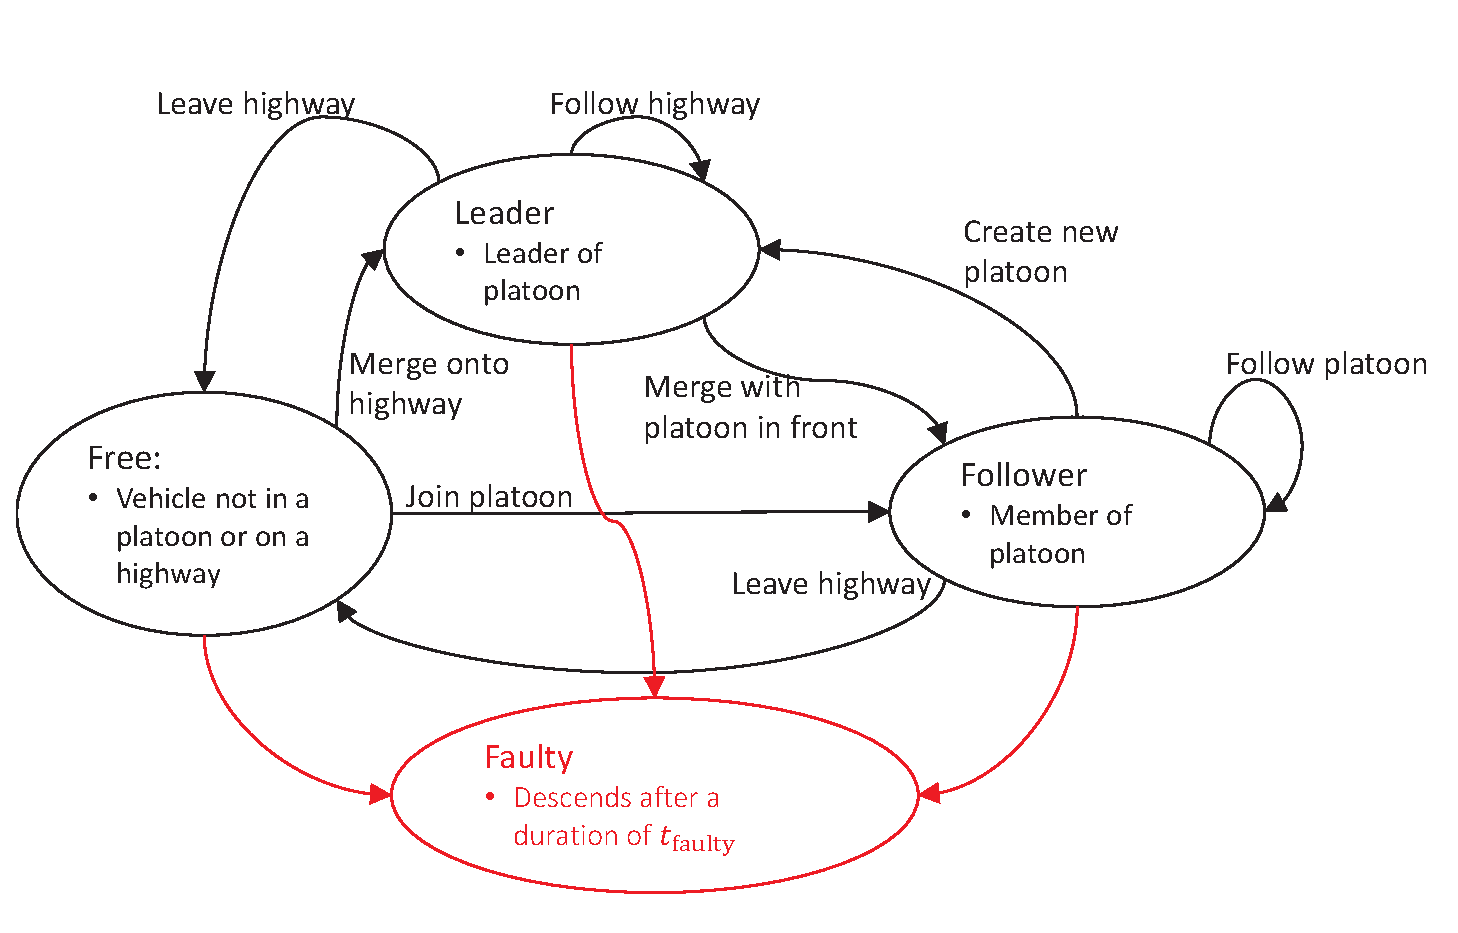
\includegraphics[width=0.5\textwidth]{fig/vehicleModes}
	\caption{Hybrid modes for vehicles in platoons.}
	\label{fig:vehicleModes}
\end{figure}

\subsection{Objectives}
Using the previously-mentioned modeling assumptions, we would like to address the following questions:

\begin{enumerate}
\item How can vehicles effectively form platoons?
\item How can the safety of the vehicles be ensured during normal operation and when there is a malfunctioning vehicle within the platoon?
\item How can the platoon respond to intruders such as unresponsive UAVs, birds, or other aerial objects?
\end{enumerate}

The answers to these questions can be broken down into the maneuvers listed in Section \ref{subsec:platoon_def}. In general, the control strategies of each vehicle have a liveness component, which specifies a set of states towards which the vehicle aims to reach, and a safety component, which specifies a set of states that it must avoid. In this paper, we address both the liveness and safety component using reachability analysis.